\documentclass[]{article} 
\usepackage{proceed2e}

\usepackage[numbers,sort]{natbib}
\usepackage{amsmath}
\usepackage{amssymb}
\usepackage{graphicx}
\usepackage{ifthen,version}
\newboolean{include-notes}
\usepackage{algorithm}
\usepackage{algpseudocode}
\usepackage[usenames,dvipsnames]{color}
\newcommand{\stnote}[1]{\textcolor{Blue}{\textbf{ST: #1}}}



\title{Planning with Affordances}

\begin{document}
\author{}
\maketitle

\begin{abstract}
Current methods for decision-making under uncertainty require
exhaustive enumeration of all possible states and actions, leading to
exponential run times caused by the well-known ``curse of
dimensionality.''  Approaches to address this problem by providing the
system with formally encoded knowledge such as options or
macro-actions still fail to prevent the system from considering many
actions which would be obviously irrelevant to a human solving the
same problem.  To address this issue, we introduce a novel approach
which represents knowledge about the domain in terms of {\em
  affordances}~\citep{gibson77}.  Our affordance formalism and
associated planning framework allows an agent to efficiently prune its
action space based on domain knowledge.  This pruning significantly
reduces the number of state/action pairs the agent needs to evaluate
in order to act optimally.  We demonstrate our approach in the
Minecraft domain on several planning and building tasks, showing a
significant increase in speed and reduction in state-space exploration
compared to subgoal (partial order) planning.
% options, and macro actions
\end{abstract}

%\stnote{High level things we should add:
%\begin{itemize}
%\item Runtime of the three algorithms in big O notation.
%\item Results with non-deterministic T.
%\end{itemize}
%}

\section{INTRODUCTION}

As robots move out of the lab and into the real world, planning
algorithms need to be able to scale to domains of increased noise,
size, and complexity.  A classic formalization of this issue is the
sequential decision making problem, where increases in problem size
and complexity directly correspond to an explosion in the state-action
space. Current approaches to solving sequential decision making
problems cannot tackle these problems as the state-action space
becomes large~\citep{grounds05}.

To address this state-space explosion, prior work has explored adding
knowledge to the planner to enable it to solve problems in these
massive domains. Humans provide an excellent existence proof for such
planning, as we are capable of searching over an immense number of
possible actions when presented with a goal.  However prior approaches
such as options and macro-actions work by providing additional
high-level actions to the agent, which {\em increases} the size of the
state/action space (while also allowing the agent to search more
deeply within the space).  The resulting augmented space is even
larger, which has the paradoxical effect of increasing search times.

\begin{figure}
\centering
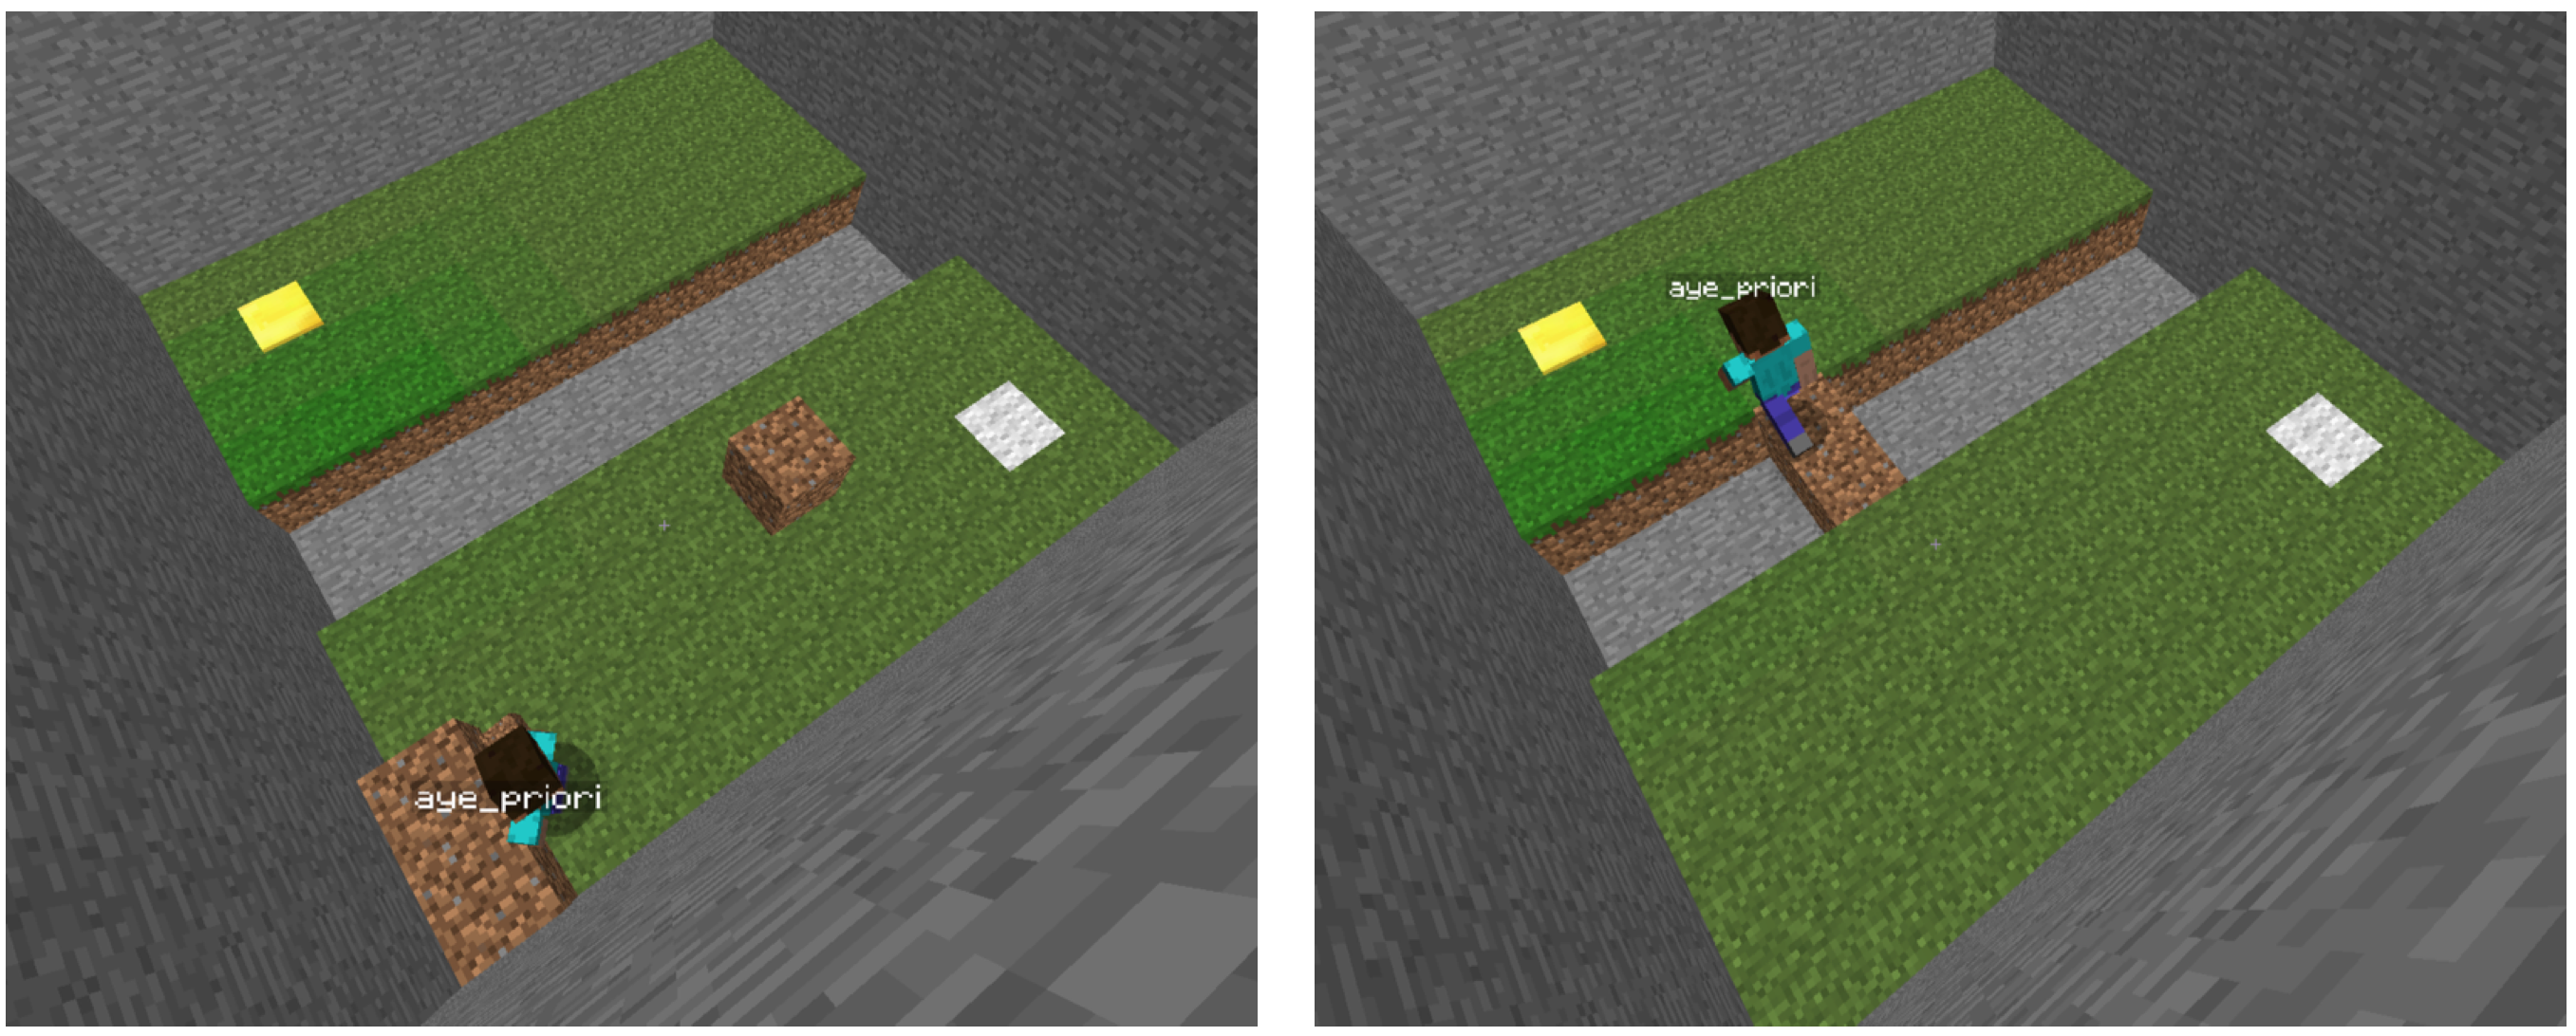
\includegraphics[scale =0.18]{figures/bridgeworld_vi_vs_aff.png}
  \caption{Classic Value Iteration (left) compared to the Affordance planner (right) in a bridge building task.}
  \label{fig:minecraft}
\end{figure}

One approach to explaining how humans solve this planning problem is
by focusing on problem-specific aspects of the environment which focus
the search toward the most relevant and useful parts of the
state-action space.  This alternative approach aims to {\em reduce}
the size of the state action space, leading to dramatic speedups in
planning.  Our approach is a formalization of {\em affordances},
introduces by \citet{gibson77} as ``what [the environment] offers [an]
animal, what [the environment] provides or furnishes, either for good
or ill.''  

In this paper we will formalize the notion of an affordance as a piece
of planning knowledge provided to an agent operating in a Markov
Decision Process (MDP)~\citep{kaelbling99}.  We demonstrate that, like
an option or macro-action, an affordance provides additional
information to the agent, enabling more transferable and efficient
planning.  However, unlike previous approaches, an affordance enables
more significant speedups by reducing the size and branching-factor of
the search space, enabling an agent to focus its search on the most
relevant part of the problem at hand.  This approach means that a
single set of affordances provides general domain knowledge, becoming
relevant just when the agent reasons that it needs to pursue a
particular goal.  Furthermore, affordances are not specific to a
particular reward function or goal, and thus, provide the agent with
transferrable knowledge that is effective in a wide variety of
problems.


\begin{figure}
\centering
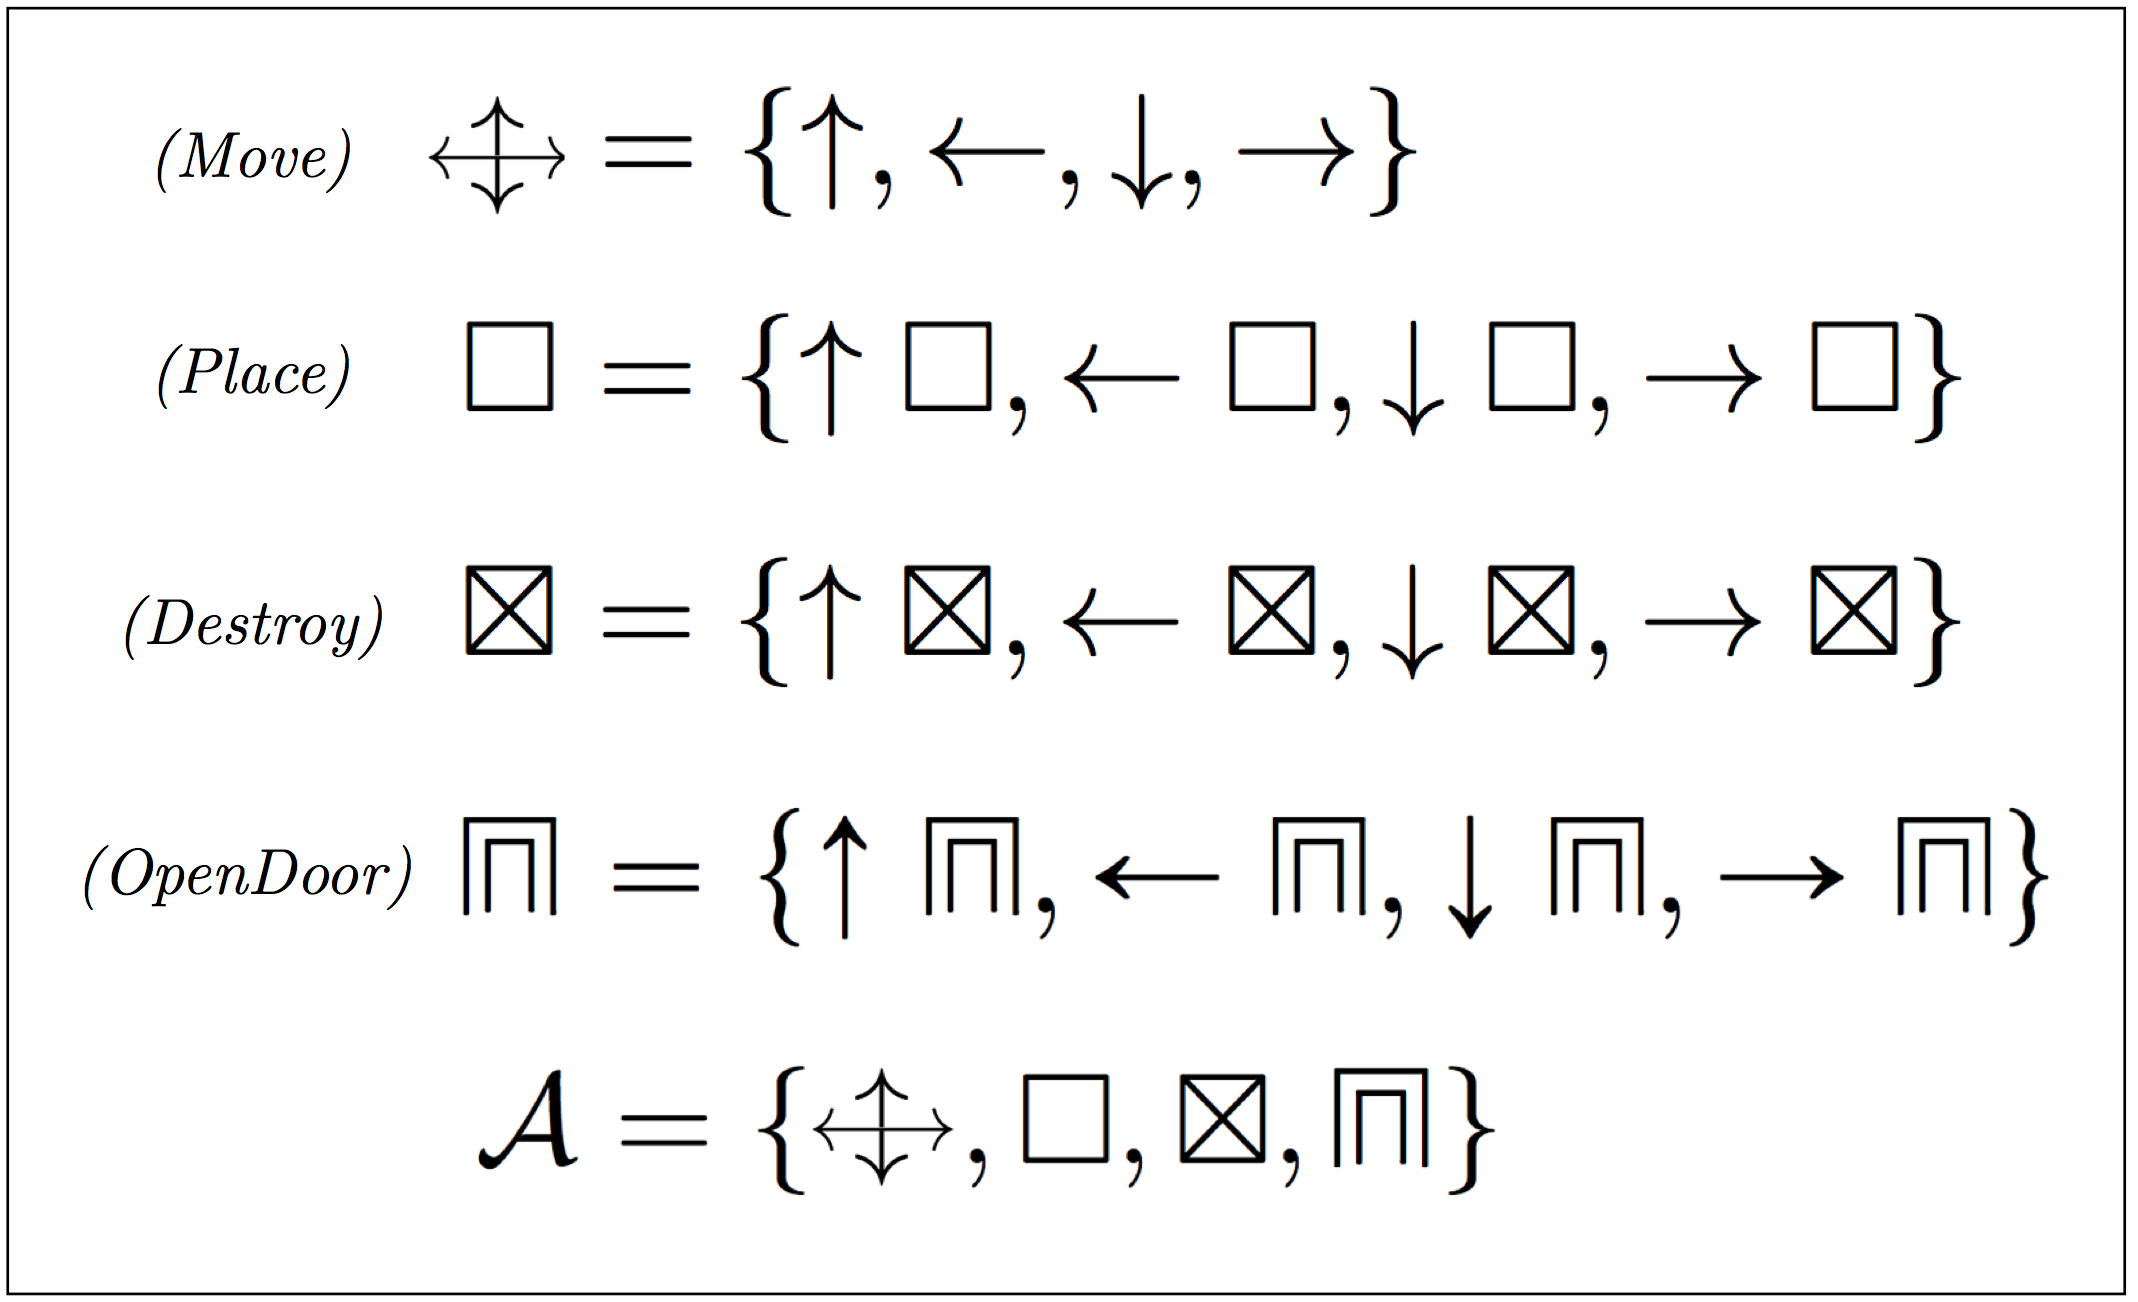
\includegraphics[scale = 0.15]{figures/all_actions.png}
\caption{The set of all actions in the Minecraft domain. \label{fig:all_actions}}
\end{figure}

\section{BACKGROUND}

We define affordances in terms of an Object Oriented Markov Decision
Process (OO-MDP)~\citep{diuk08} and review competing approaches for
adding knowledge to planning.

\subsection{DOMAIN}

We will be using Minecraft as our primary planning and evaluation domain. Minecraft
is a 3-D block world game in which the user can place and destroy blocks of
different types. As a running example, we will consider the problem of an agent
attempting to cross a trench in a $4 \times 4 \times 2$ Minecraft world shown
in Figure~\ref{fig:bridgeworld}. The floor (at $z = 1)$ \footnote{The $z$-axis
is the height of the Minecraft world. Similarly, the $x$-axis is its width and the
$y$-axis is its length.} is composed of 8 solid blocks, with horizontal empty
trenches at $y = 2$ and $y = 3$. The agent is  at the starting location
$(1, 1, 2)$ and needs to reach the goal at $(4,4,2)$

To solve the problem, the agent must
place a block in the trench to form a bridge, then cross the bridge
to reach the goal.  However, when running an uninformed planning
technique such as value iteration, the agent must enumerate all
possible states, such as placing a block in the corner and
subsequently destroying it.  Considering these actions (which are
obviously irrelevant to a human player) results in a combinatoric
explosion of the state space (see Equation \ref{eq:mc_explode}).

\subsection{OO-MDP}

OO-MDPs are an extension of the classic Markov Decision Process (MDP).
A finite MDP is a five-tuple: $\langle \mathcal{S}, \mathcal{A},
\mathcal{T}, \mathcal{R}, \gamma \rangle$, where $\mathcal{S}$ is a
state-space, $\mathcal{A}$ is the agent's set of actions,
$\mathcal{T}$ denotes $\mathcal{T}(s' \mid s,a)$, the transition
probability of an agent applying action $a \in \mathcal{A}$ in state
$s \in \mathcal{S}$ and arriving in $s' \in \mathcal{S}$, and
$\mathcal{R}(s,a)$ denotes the reward at $s$ when action $a$ is
applied, and $\gamma$ is a discount factor.

\begin{figure}
\centering
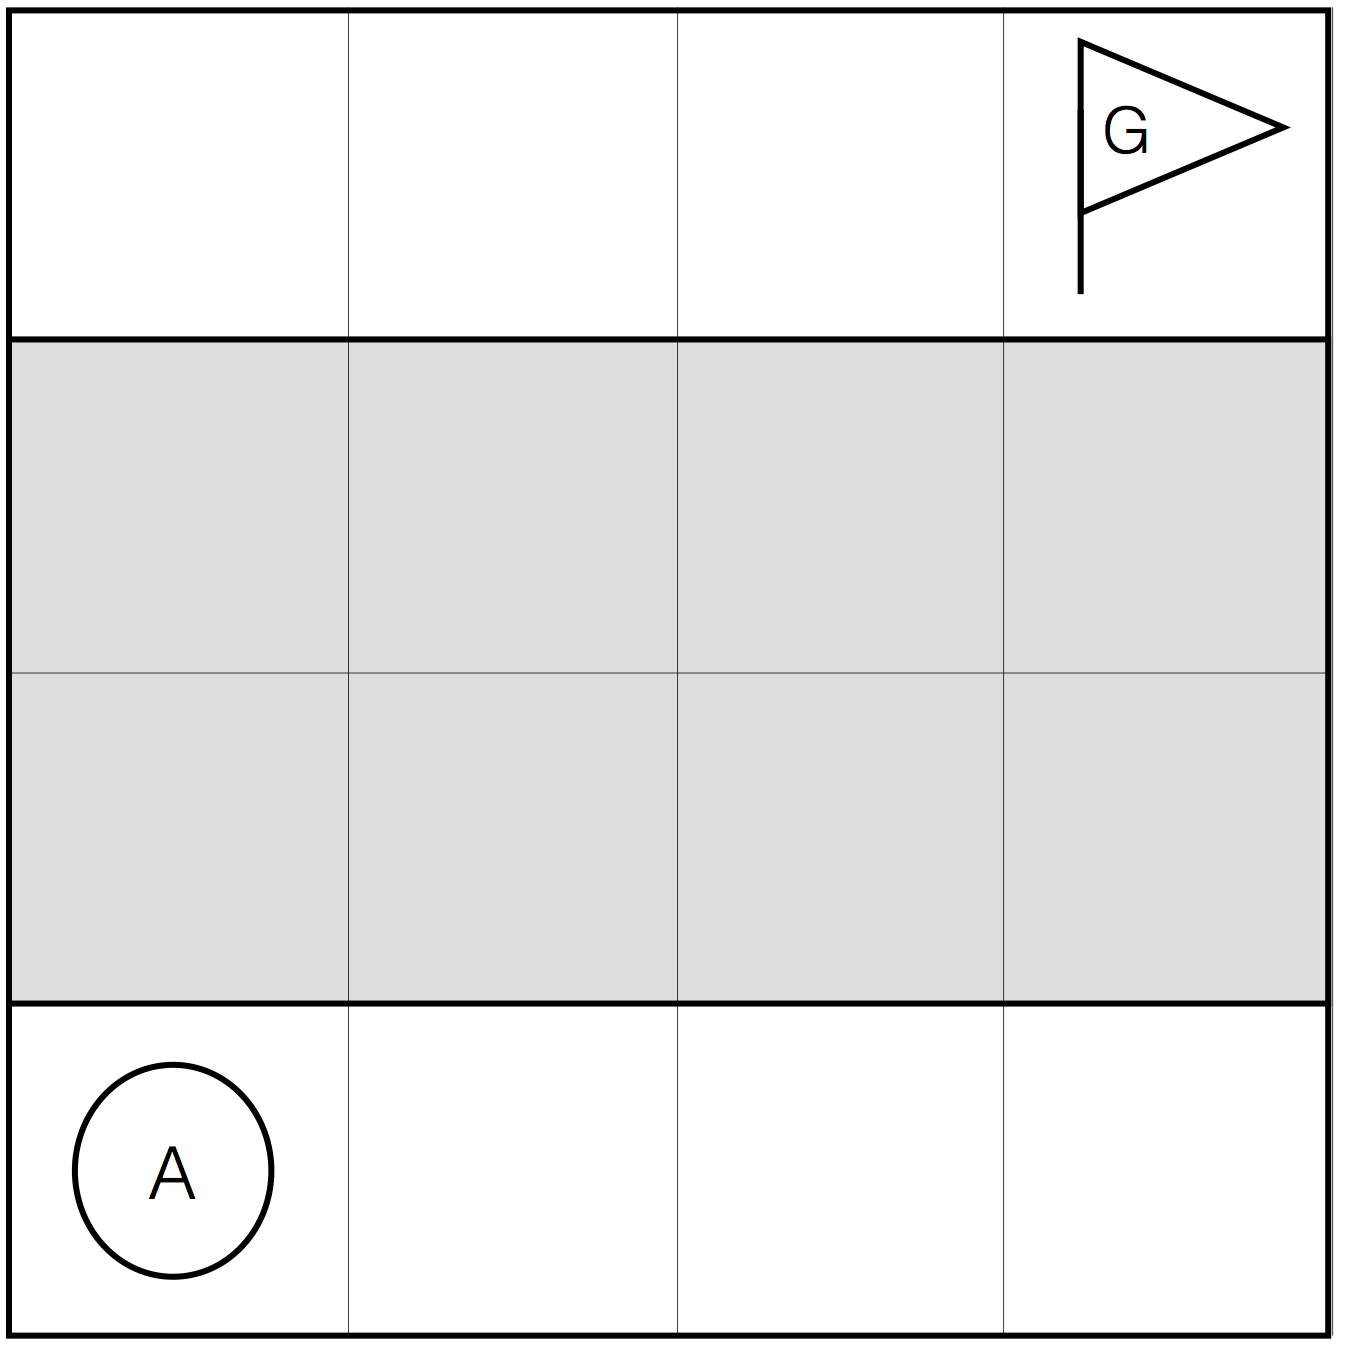
\includegraphics[scale=0.2]{figures/bridgeworld.png}
\caption{In the above Minecraft planning problem \texttt{BRIDGEWORLD},
the agent must place a block in the trench in order to reach the goal 
(the trench is too wide to jump over). \label{fig:bridgeworld}}
\end{figure}

A OO-MDP represents the state space as a collection of objects,
$O = \{o_1, \ldots, o_o \}$.  Each object $o_i$ has a
class $c_j \in  \{c_1, \ldots, c_c\}$. Every class has a set of attributes
$Att(c) = \{c.a_1, \ldots, c.a_a \}$, each of which has a domain $Dom(c.a)$.
Upon instantiation of an object its attributes are given a state $o.state$
(an assignment of values to its attributes).  Finally, the underlying MDP is the union
of all the states of its objects $\cup_{i = 1}^o o_i.state$. ~\citep{diuk08}

Our motivation for using an OO-MDP instead of an MDP lies in the
ability to formulate predicates over classes of objects. As we will
see in section 3, this helps us form preconditions and goals that
generalize beyond a particular instance of a state space.

As with a classical finite MDP, planning with an OO-MDP involves
running value iteration to determine a policy.  Reward propagation in
value iteration occurs as in a Bellman update:
\begin{align}
U_{i+1}(s) \leftarrow \mathcal{R}(s) + \gamma \max_{a \in \mathcal{A}(s)} \sum_{s'} \text{Pr}(s' \mid s, a)U_i(s')
\end{align}
Where $U_i(s)$ is the {\it utility} of state $s$ at iteration $i$, 
representing the expected reward of being in that state. See Algorithm \ref{alg:vi} for the full pseudocode of the algorithm ~\citep{russellnorvigAI}.

% VI pseudocode from Norvig/Russell
\begin{algorithm}
  \caption{Value-Iteration($\mathcal{A}$, $\mathcal{R}$, $\mathcal{S}$, $\epsilon$, $\gamma$) \\ {\it Complexity:} $\mathcal{O}(|\mathcal{A}|\cdot |\mathcal{S}|^2)$}
  \begin{algorithmic}[1]
    \While {$\delta < \epsilon \frac{(1-\gamma)}{\gamma}$}
    \State $U \gets U';\delta \gets 0$
    \For {each state $s \in \mathcal{S}$}
    \State $U'[s] \leftarrow \mathcal{R}(s) + \gamma \max_{a \in \mathcal{A}(s)} \sum_{s'} \text{Pr}(s'\mid s,a) U[s']$
    \If {$|U'[s] - U[s]| > \delta$}
    	\State $\delta \gets |U'[s] - U[s]|$ 
    \EndIf
    \EndFor
    \EndWhile \\
    \Return U;
  \end{algorithmic}
  \label{alg:vi}
\end{algorithm}


In practice, Value Iteration scales very poorly, either as the state
space grows, or the action set grows. This is because the state-action
space, depending on the domain, grows exponentially in the number of
actions.  This problem is ameliorated slightly by introducing the
OO-MDP, but it still fails in just about all of the planning scenarios
we introduce here because the agent explores all states that result
from applying every action in every state.  The complexity of Value-Iteration
is known to be $\mathcal{O}(|\mathcal{A}||\mathcal{S}|^2)$, so as the number
of states increases, the runtime of Value Iteration grows quite quickly.

\subsection{SUBGOALS}

Subgoal planning leverages the intuition that certain goals in
planning domains may only be brought about if certain preconditions
are first satisfied. For instance, in the bridge problem, one must
first place a block in the trench to create a bridge before crossing
the trench.  \citet{branavan12a} explore learning subgoals from the
Minecraft wiki and applying them in order to plan through a variety of
problems in Minecraft.  

% Formalism
Formally, in subgoal planning, the agent is set of subgoals, where each subgoal is a pair of predicates:
\begin{align}
SG = \langle x_k, x_l \rangle
\end{align}

where $x_l$ is the effect of some action sequence performed on 
a state in which $x_k$ is true. Thus, subgoal planning requires 
that we perform high-level planning in subgoal space, and low-level 
planning to get from subgoal to subgoal. The low-level planner may vary, though
Metro-FF is a popular choice, as is Value Iteration.

% Subgoal planning pseudocode
\begin{algorithm}
  \caption{Plan with Knowledge Base of Subgoals \\ {\it Complexity:} $\mathcal{O}(|\mathcal{A}|\cdot |\mathcal{S}|^2)$}
  \begin{algorithmic}[1]
    \State subgoalSequence $\gets$ BFS(subgoalKB, goal)
    \State plan = []
    \State curState $\gets$ subgoalSequence.pop()
    \For {subgoal $\in$ subgoalSequence}
    		\State plan += ValueIteration(curState, subgoal)
		\State curState $\gets$ plan.getLastState()
    \EndFor \\
    \Return plan;
  \end{algorithmic}
\end{algorithm}

In the case of \texttt{BRIDGEWORLD}, the agent might consider placing
a block somewhere along the trench to be a subgoal. Then, it runs
Value Iteration to get from its starting location to the subgoal.
Next, it runs Value Iteration from the first subgoal to the finish.
Subgoals enhance an agent's planning abilities when they propose {\it
  necessary} claims about the domain. If the subgoals are {\it
  contingent} (i.e. true in some state spaces of the domain but not in
others), then they do not limit the search space. For instance,
consider the task in \texttt{BRIDGEWORLD}, in which the agent must
place a block in the trench that separates the agent from the goal.
The subgoal $\langle blockInTrench, reachGoal\rangle$ might be a
perfectly useful subgoal in \texttt{BRIDGEWORLD}, but an adversary
could easily come up with thousands of worlds in which such a subgoal
would completely derail the agent's planner. Thus, many subgoals do
not scale beyond a particular instance of a state space. In order for
subgoals to be useful, they must be necessary claims about the domain,
otherwise, one can always come up with a counter world (by definition
of necessary).  Compare this scenario to the problem of baking bread
in minecraft: posessing wheat is always required to make bread, and it
is impossible to construct a world where this precondition is not
true.

{\bf Problem 2: Efficient Search} The last problem with subgoal
planning is that the use of subgoals actually requires that we
research a huge portion of the state space. Consider the
\texttt{BRIDGEWORLD} example in which the subgoal is to place a block
along the trench somewhere - once we plan from the state in which a
block has been placed at the trench, Value Iteration will search paths
exploring both sides of the trench rather than focusing on the
opposite side of the trench toward the goal.

\begin{figure}
\centering
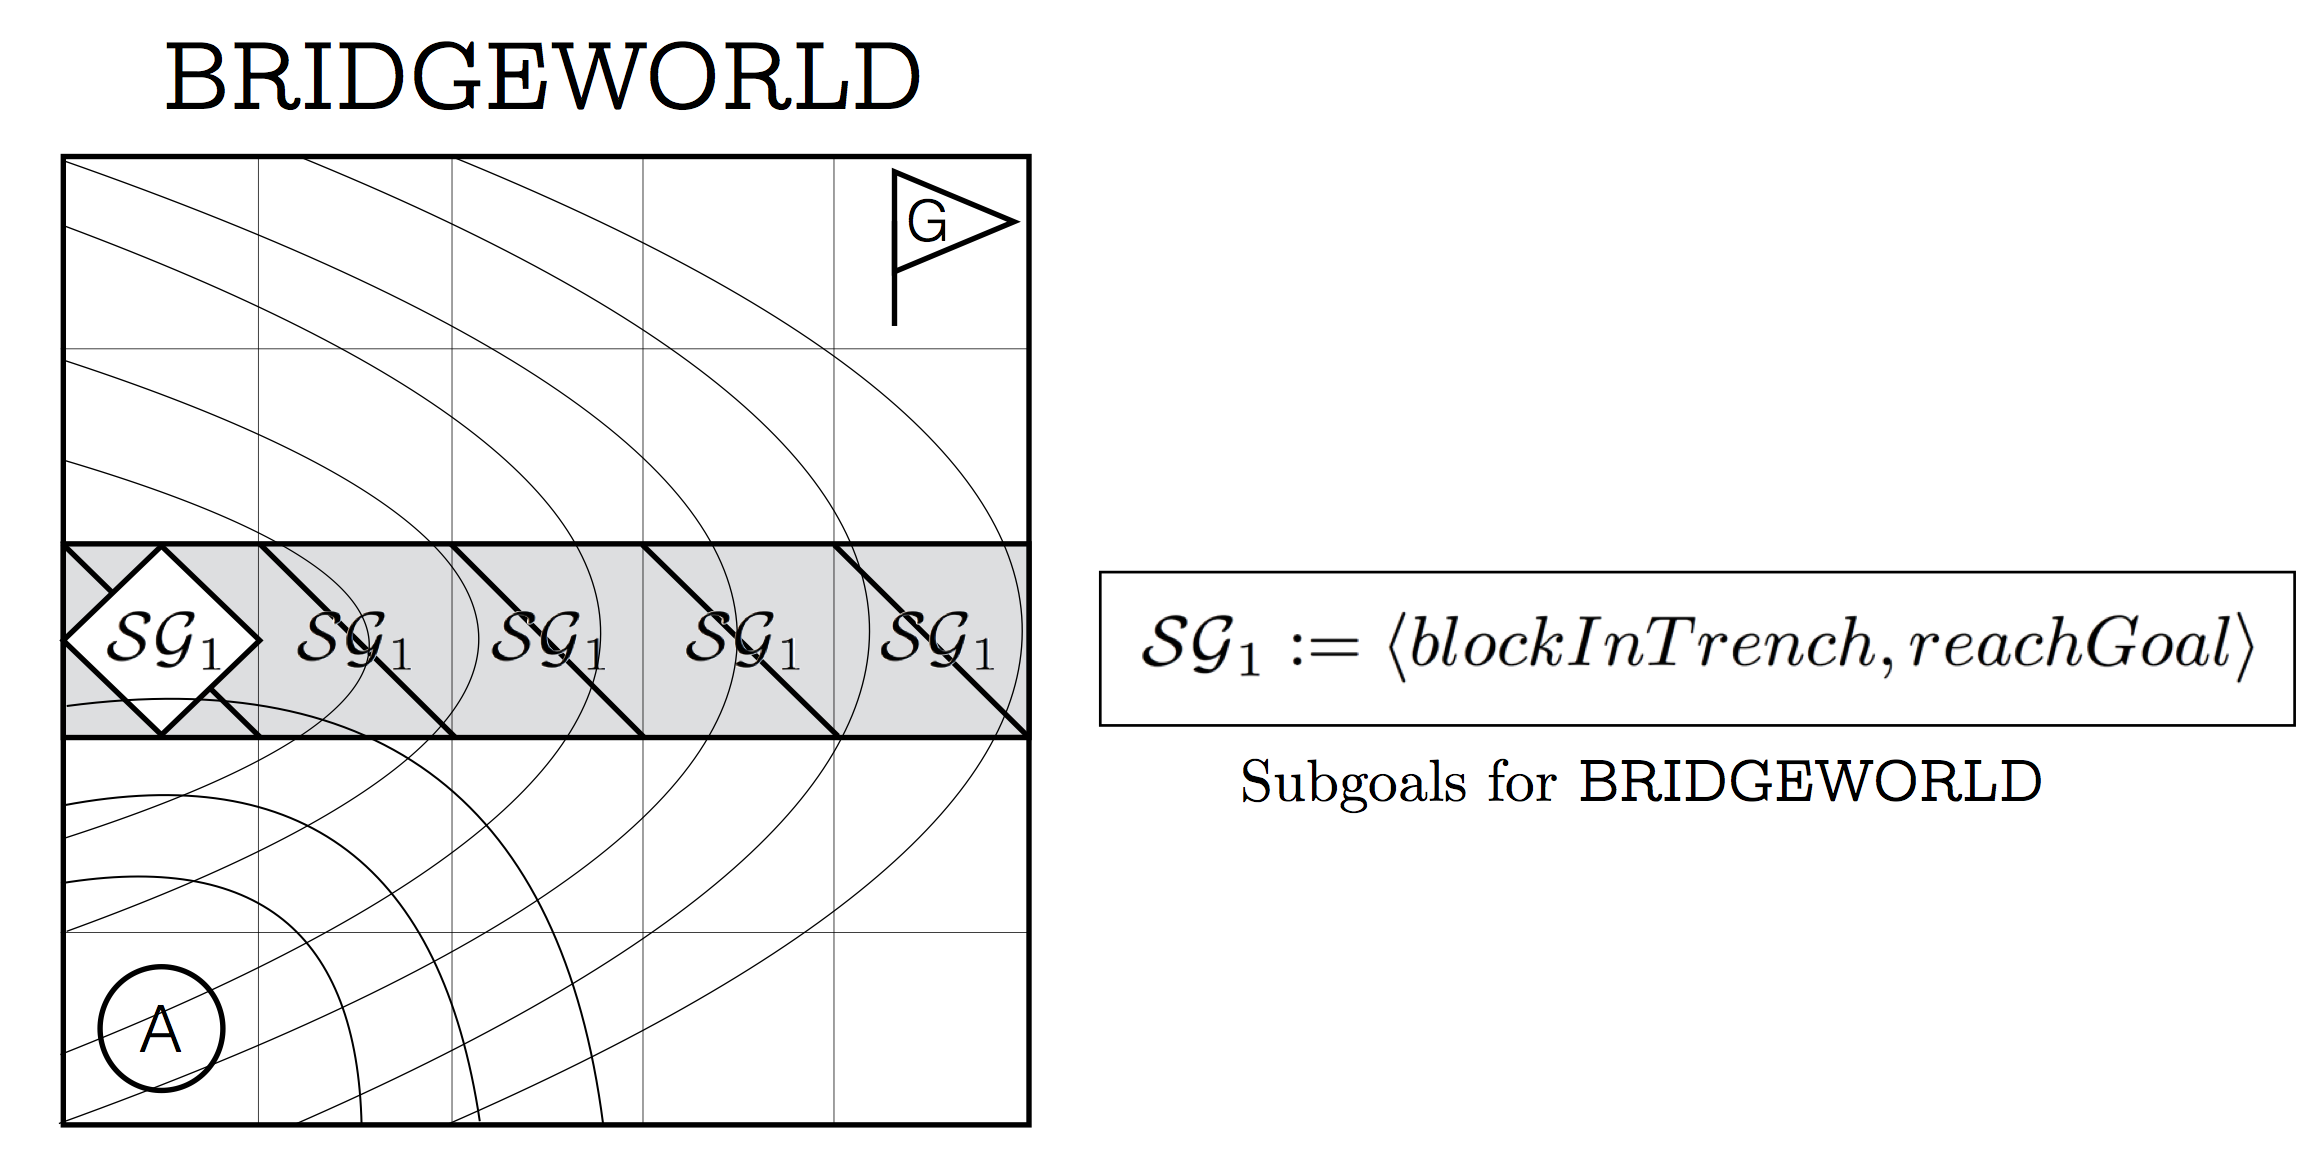
\includegraphics[scale=0.22]{figures/bridgeworld_sg.png}
\caption{The agent re-explores a large portion of the state space 
once it finds $\mathcal{SG}_1$. Also note that this subgoal 
highlights {\bf Problem 1}, in that it would be useless in many other Minecraft state spaces.}
\label{fig:bwsg}
\end{figure}


A final, but less significant problem, is that Subgoal planning still 
requires the use of Value Iteration or another low-level planner, which does not scale well - if 
there is ever a case in which planning between two subgoals is 
at all complex, then Subgoal planning is out of luck.

\subsection{OPTIONS}

The options framework proposes incorporating high-level policies to 
accomplish specific sub tasks. For instance, when an agent is near 
a door, the agent can engage the `door-opening-option-policy', which 
switches from the standard high-level planner to running a policy 
that is hand crafted to open doors. An option $o$ is defined as follows:

$o\ =\ \langle \pi_0, I_0, \beta_0\rangle$, where:

\begin{itemize}
\item[] $\pi_0 : (s,a) \rightarrow [0,1]$
\item[] $I_0 : s \rightarrow \{0,1\}$
\item[] $\beta_0 : s \rightarrow [0,1]$
\end{itemize}

Here, $\pi_0$ represents the {\it option policy}, $I_0$ represents
a precondition, under which the option policy may initiate, and 
$\beta_0$ represent the post condition, which determines which 
states terminate the execution of the option policy.

As Konidaris and Barto point out, the classic options framework is not 
generalizable, as it does not enable an agent to transfer knowledge from 
one state space to another. Recently, Konidaris and Barto's ~\citep{konidaris07} 
expand on the classic options framework and allow for a more portable 
implementation of options. Still, though, planning with options requires either 
that we plan in a mixed space of actions {\it and} options (which blows up the 
size of the search space), or requires that we plan entirely in the space of options. 
Additionally, providing an agent with an option policy is a difficult task for a human 
designer (especially if we want an optimal policy, which we do).

\subsection{MACROACTIONS}

\[
\boxed{\text{Running Example}}
\]

\section{AFFORDANCES}

%% Formalism
We define an affordance, $\Delta$, as a tuple, $\langle
p,g\rangle\ \longrightarrow \alpha$, where:
\begin{itemize}
\item[] $\alpha$ is a subset of the action space, $\mathcal{A}$
\item[] $p$ is a predicate on states, $s \longrightarrow \{$0$, 1\}$
  representing the {\em precondition} for the affordance.
\item[] $g$ is a predicate on states, $s \longrightarrow \{$0$,1\}$
  representing the {\em postcondition}.
\end{itemize}

The intuition behind an Affordance is that in a huge number of planning 
scenarios, not all actions are needed in all states. In fact, many applications 
of actions in states do not contribute toward solving the planning task, but 
instead, cause the state-space to grow exponentially. This is especially true 
in domains in which the agent's actions can drastically shape the environment, 
such as in Minecraft. Thus, Affordances are used in order to determine which 
actions are relevant in which states, given a specific goal. For instance, if the 
agent is at the trench in \texttt{BRIDGEWORLD} and trying to reach the goal then it
would not consider destroying a block, as that does not further its ability
to reach the goal. Eliminating the ``destroy" action avoids 
exploring every consequent state in which that block has been destroyed.

The Affordance Value-Iteration algorithm (for full pseudocode see Algorithm \ref{alg:aff_vi}) works by
only enumerating a subset of the actual state space. More specifically, the state space is generated
outward from the agent's start state by applying actions that are deemed relevant by the current
set of affordances. Thus, in most cases, a much smaller state space $\hat{\mathcal{S}}$ is produced,
on which Value-Iteration finds an optimal policy.

The predicate $p$ and goal $g$ that are constituents of an Affordances are both subsets of the union
of object states $\cup_{i = 1}^o o_i.state$ (see section 2.2).  The use of an OO-MDP gives us easy access to these
robust predicates which completely describe the underlying MDP in a much more general manner.

The primary benefit of encoding goal relative knowledge in each Affordance
is that actions may be pruned with respect to a given goal. As a result,
agents may be endowed with huge action sets that enables them to solve a variety of
problems across variable state-spaces. This
hints at the transferability that we will demonstrate empirically in the next section.

\begin{figure}
\centering
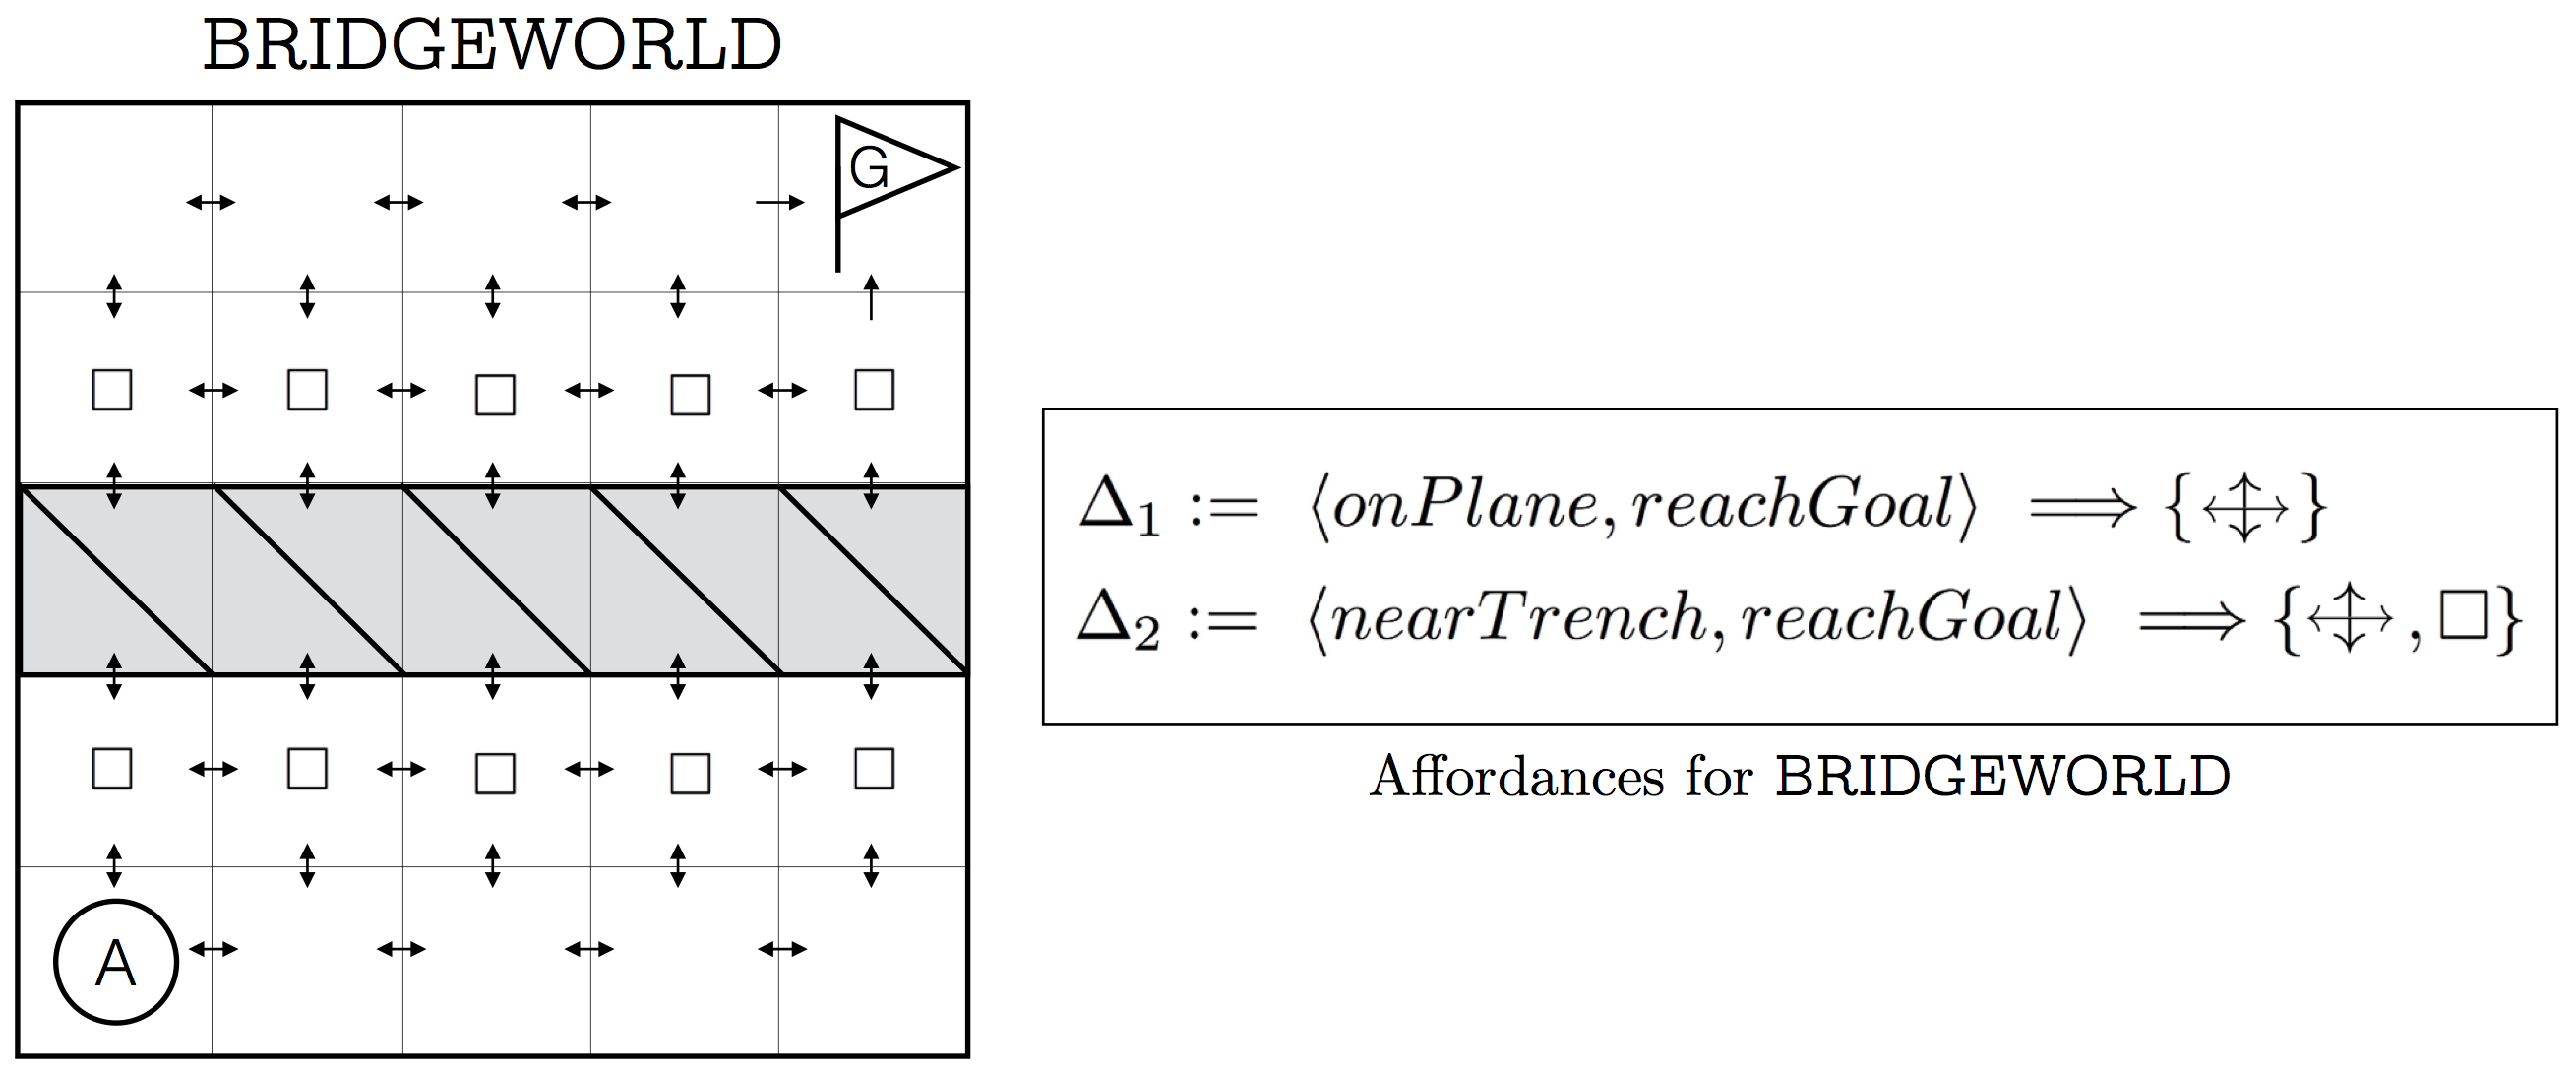
\includegraphics[scale=0.22]{figures/bridgeworld_aff.png}
\caption{The Affordance planner's state-action space on \texttt{BRIDGEWORLD}.}
\label{fig:bridgeworld_aff}
\end{figure}

Furthermore, given perfect subgoal knowledge for a
particular planning task, the affordance formalism will find an
optimal policy {\it extremely} quickly. We imagine extensions in which
an agent gets stuck and must ask a human partner for help using
natural language, and the resulting dialogue could endow the agent
with subgoal knowledge. This also allows the agent to prune way
unnecessary actions in $\mathcal{A}$ in each specific planning task,
making it possible to solve a engage with a large number of planning
scenarios that may call for different actions. 


% VI pseudocode + Affordances
\begin{algorithm}
  \caption{Affordance-VI($\mathcal{A}$, $\mathcal{R}$, $s_0$, $kb$, $goal$, $\epsilon$, $\gamma$) \\ {\it Complexity:} $\mathcal{O}(|\mathcal{A}|\cdot |\hat{\mathcal{S}}|^2)$}
  \begin{algorithmic}[1]
    \State $\hat{\mathcal{A}} \gets pruneActions(kb, s_0, \mathcal{A}, goal)$
    \State $\hat{\mathcal{S}} \gets genStates(kb, \hat{\mathcal{A}})$
    \While {$\delta < \epsilon \frac{(1-\gamma)}{\gamma}$}
    \State $U \gets U';\delta \gets 0$
    \For {each state $s \in \hat{\mathcal{S}}$}
    \State $U'[s] \gets \mathcal{R}(s) + \gamma \max_{a \in \hat{\mathcal{A}}(s)} \sum_{s'} \text{Pr}(s'\mid s,a) U[s']$
    \If {$|U'[s] - U[s]| > \delta$}
    	\State $\delta \gets |U'[s] - U[s]|$ 
    \EndIf
    \EndFor
    \EndWhile\\
    \Return U;
  \end{algorithmic}
  \label{alg:aff_vi}
\end{algorithm}

In the worst case, the Affordance-Value-Iteration Algorithm is 
bounded by $\mathcal{O}(|\mathcal{A}|\cdot |\hat{\mathcal{S}}|^2)$, where
$\hat{\mathcal{S}}$ is the subset of the states that were reachable using the
resulting pruned action set determined by the agent's affordances. Thus,
if the affordances were poorly designed, then the lower bound for the size of
$\hat{\mathcal{S}}$, is precisely the full state space, $\mathcal{S}$. However,
in general, when reasonable affordances are applied the agent is guaranteed to prune its
action set for any number of states, and thus will explore less of the state space
as a result.

The affordance formalism introduced above and expanded on in this
paper resolves the weaknesses of these other frameworks by limiting
the complexity of the seed knowledge required of the designer, while
still providing enough knowledge to limit the search space but also
maintain scalability.

\section{EXPERIMENTS}

%\stnote{To write the experiments section, it's good to say what we are
%  interested in learning first.  What are we testing?  What is our
%  hypothesis?  Then explain the setup, then explain what the results
%  say about the hypothesis.  I would make experiments and results one
%  section, with subsections for each experiment + results}

We conducted a series of experiments in the Minecraft domain that
tested each planning system on a variety of tasks, ranging from basic
path planning, to baking bread, to opening doors and jumping over
trenches.  We also tested each planner on worlds of varying size to
demonstrate the scalability of each system. In Table \ref{results_1},
we provide results on testing the planners across each system. For
each data point, we ran the planning system 3 times and took the
average result (they rarely deviated beyond $\frac{1}{10}$ of a
second).

For the scenarios listed in Table \ref{results_1}, we limited the agent's 
action set across all planners so that it did not have access to block 
placement ($\square$) and block destruction ($\boxtimes$). The reason 
for excluding these two action types up is that, in Minecraft, the agent 
has an extraordinary ability to modify the state space via placing and 
destroying blocks. As a result, if an agent begins placing or destroying 
blocks in cases where it does not need to, the state-action space will 
explode exponentially and grow far too fast for (almost) any planner to 
finish in our lifetime. 

Consider that the agent is capable of destroying and placing blocks 
in a 10x10x2 world; there are on the order of:

\begin{align}
O\left(\sum_{n=1}^{10 \cdot 10 \cdot 2} \binom{10 \cdot 10 \cdot 2}{n}\right)
\label{eq:mc_explode}
\end{align}

states, which is far too large to explore. We will demonstrate that our 
affordance model {\it is} capable of handling these types of actions, 
and can plan using them as in a bridge building scenario or tunnel 
digging scenario (among others) while the other planners cannot. 
In fact, with these actions, none of the other planning systems 
can solve even the most basic path planning (even on just a flat 
surface with no obstacles). We explore this ability in the results 
seen in Table \ref{results_2}

As discussed above, one of the major advantages of using Affordances 
to plan is that they enable an agent to have a massive action set, 
making Affordances effectively transfer between domains. We 
conducted an additional set of experiments on the 15x15 world 
with no obstacles \texttt{15WORLD}. For this round of testing, we 
varied the number of actions available to the agent (starting from 
$|\mathcal{A}| = 4$ up to $|\mathcal{A}| = 25$) and ran the planner 
on \texttt{15WORLD} with the same goal (to reach the goal in the corner).


An additional advantage of planning with Affordances is that the 
problems of block-placement and block-destruction illustrated by 
\ref{eq:mc_explode} are overcome. With Affordances, we are able 
to solve a variety of novel planning problems in the Minecraft 
domain, such as building a bridge to cross a long trench, or digging 
a hole through a wall to reach the goal (see Table \ref{results_2}). 
This is indeed a compelling result, as no other planning system is 
currently able to avoid falling prey to the state-space explosion 
mentioned above. Additionally, the malleability of Minecraft that 
causes this explosion is a reasonable model of the way that an 
agent in the real world is capable of modifying its surroundings. 
Thus, we foresee the Affordance planner as being extremely deft 
at handling real world planning scenarios.

\section{RESULTS}

\begin{table}
\begin{tabular}{ l || c | c | c }
  & Affordances & Subgoals & VI \\
  \hline
  \texttt{10WORLD} 		&	{\bf 0.6s} 		&	 1.8s 		& 1.1s  \\
  \texttt{13WORLD} 		&	{\bf 2.5s} 	 	& 	10.1s 		& 6.0s  \\
  \texttt{15WORLD} 		&	{\bf 6.7s} 	 	& 	21.6s 		& 11.8s  \\
  \texttt{17WORLD} 		& 	{\bf 16.6s} 	& 	45.4s 		& 28.2s  \\
  \texttt{20WORLD} 		& 	{\bf 57.6s} 	& 	144.3s 		& 140.5s  \\
  \texttt{JUMPWORLD}  	& 	{\bf 4.3s} 		& 	21.1s 		& 10.1s \\
  \texttt{BREADWORLD}  	& 	25.5s		& 	{\bf 22.8s} 	& 51.6s \\
  \texttt{DOORWORLD}  	& 	{\bf 16.3s} 	& 	25.0s 		& 25.3s \\
  \texttt{MAZEWORLD}  	& 	{\bf 17.9s} 	& 	114.8s		& 37.6s \\
  \texttt{HARDWORLD} 	& 	{\bf 34.5s}  	& 	215.9s 		& 149.7s
\end{tabular} 
\label{results_1}
\caption{Tests on a variety of tasks without block placement and destruction actions}
\end{table}

\vspace{4 mm}

\begin{table}
\begin{tabular}{ l || c | c | c }
  & Affordances & Subgoals & VI \\
  \hline
  $|\mathcal{A}| = 4$ 		& 	6.7s 	& 	11.8s 	& 6.7s  \\ % Just movement
  $|\mathcal{A}| = 8$ 		& 	6.8s 	& 	25.4s 	& 14.8s  \\ % + openDoor
  $|\mathcal{A}| = 12$ 	& 	6.8s 	& 	39.8s 	& 22.9s  \\ % + Oven
  $|\mathcal{A}| = 13$ 	& 	6.8s 	& 	41.28s      & 24.7s  \\ % + grain
  $|\mathcal{A}| = 17$ 	& 	6.7s	& 	55.5s	& 33.1s  \\ % + 0 blocks, placement
  $|\mathcal{A}| = 17$ 	& 	6.8s 	& 	DNF 		& DNF  \\ % + 1 blocks, placement
  $|\mathcal{A}| = 21$ 	& 	6.6s 	& 	DNF 		& DNF  \\ % + destruction
\end{tabular}
\label{results_2}
\caption{Plan on the simplest possible task (path planning in a flat plane with no obstacles - \texttt{15WORLD}) with incrementally larger action sets.}
\end{table}

% Should explain DNF

As one can see from Table \ref{results_2}, in those cases where
$|\mathcal{A}| = 21$ and $|\mathcal{A}| = 25$, the only planning algorithm to
actually complete the tasks was the Affordance planner. This is because each
of these cases scaled to include block destruction and block placement actions.
Thus, any case in which these actions are required to complete the task at hand,
only Affordance planning will succeed. This is significant, as Table \ref{results_1}
indicates that the Affordance planner plans more effectively than the other
systems, but it can also handle novel problems involving those actions that
alter the environment in sever ways.

We also include a Bonus round indicating
those tasks that only the Affordance planner was able to solve. Finally, since
each Affordance is attached to a particular goal, a single knowledge base will
scale across state-spaces and task types, causing Affordance planning to be
extremely transferrable. Additionally, we plan to add experiments in
Non-deterministic planning scenarios, as well as testing on the planning scenarios
from table \ref{results_1} where the knowledge bases remain constant across
state-spaces to test the generality of each algorithm.



% Insert bonus round of:
%	- Ladder!!!!
%	- Bridge
%	- Tunnel
%	- Builder tower under self

\section{CONCLUSION}

We proposed a novel approach to representing knowledge in terms of
{\em affordances}~\citep{gibson77} that allows an agent to efficiently
prune its action space based on domain knowledge. This pruning was
shown to significantly reduce the number of state/action pairs the
agent needs to evaluate in order to act optimally, and resulted in
faster planning than subgoal planning, options, and vanilla value
iteration. We demonstrated the efficacy as well as the transferability
of the affordance model in a series of planning tasks in the Minecraft
domain.

In the future, we hope to learn affordances from experience as opposed
to providing them directly to the agent. Additionally, we hope to
introduce uncertainty into the action set that is pruned, in order to
improve the effectiveness of the pruning. Lastly, we hope to
incorporate aid from a human partner through natural language
dialogue, in which the agent may ask for help when it is stuck and
receive subgoal {\it hints} from a human companion.

\bibliographystyle{plainnat}
\bibliography{main}  


\end{document}
